\subsection{Overview: high-level components and their interaction}


\begin{figure} [!h]
	\centering
	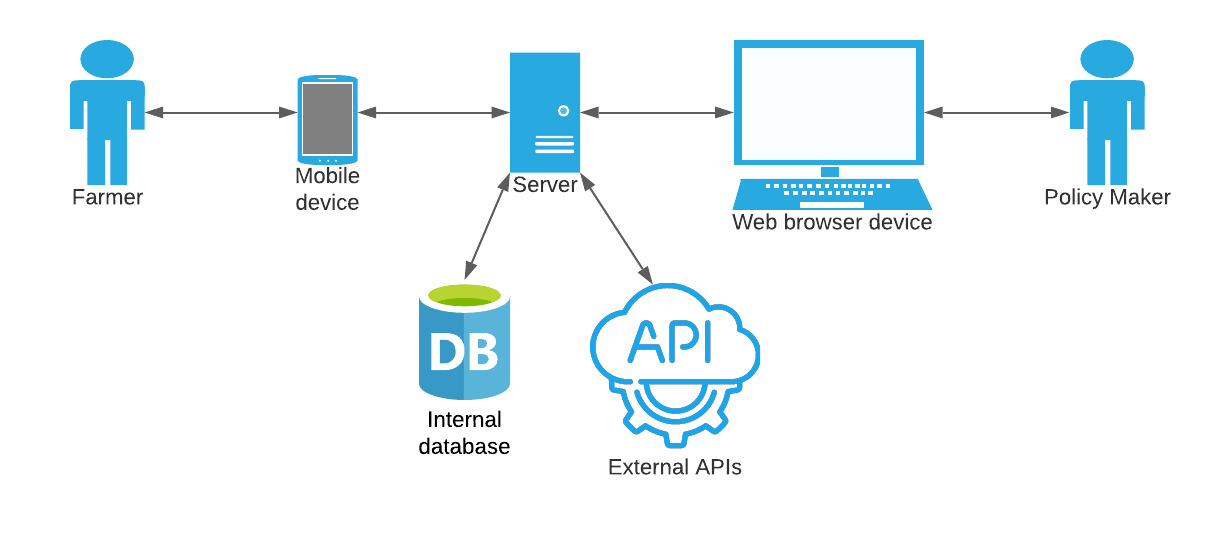
\includegraphics[width=\textwidth]{Images/architecture-diagram.png}
	\caption{\label{fig:physical_diag} Physical architecture diagram}
\end{figure}

\begin{figure} [!h]
	\centering
	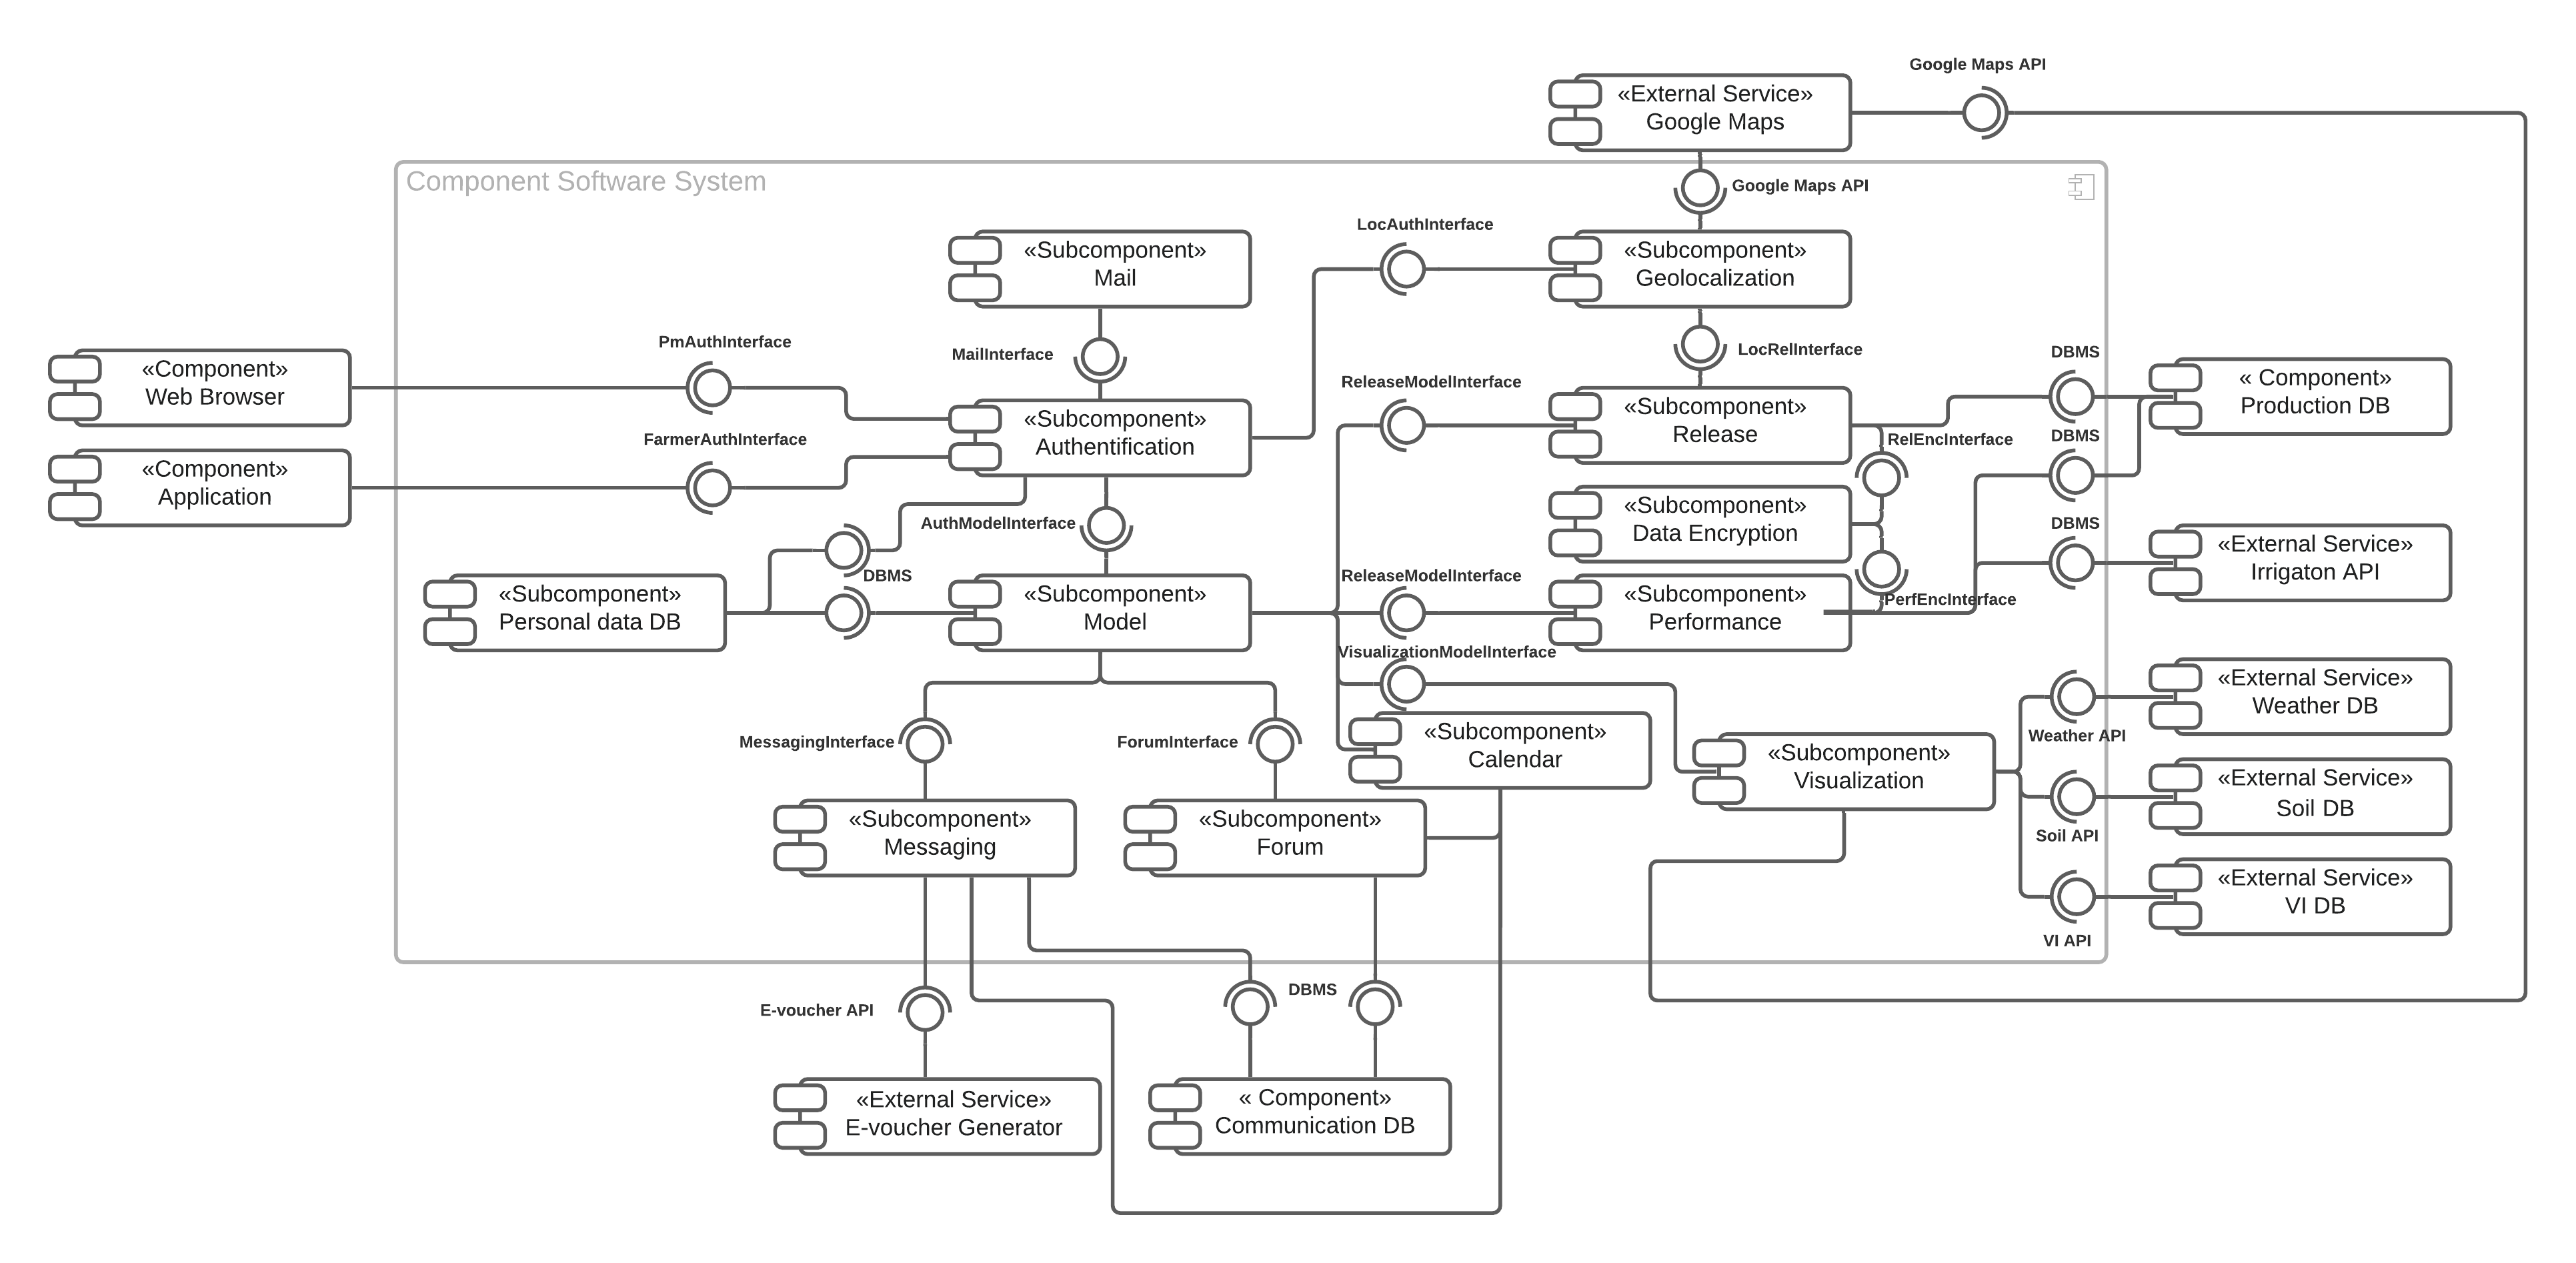
\includegraphics[width=\textwidth]{Images/component-diagram.png}
	\caption{\label{fig:component_diag} Component diagram}
\end{figure}

\subsection{Runtime view}
The following sequence diagrams aims at presenting the links between the component during the principal uses of the System by the different users.

\begin{figure} [!h]
	\centering
	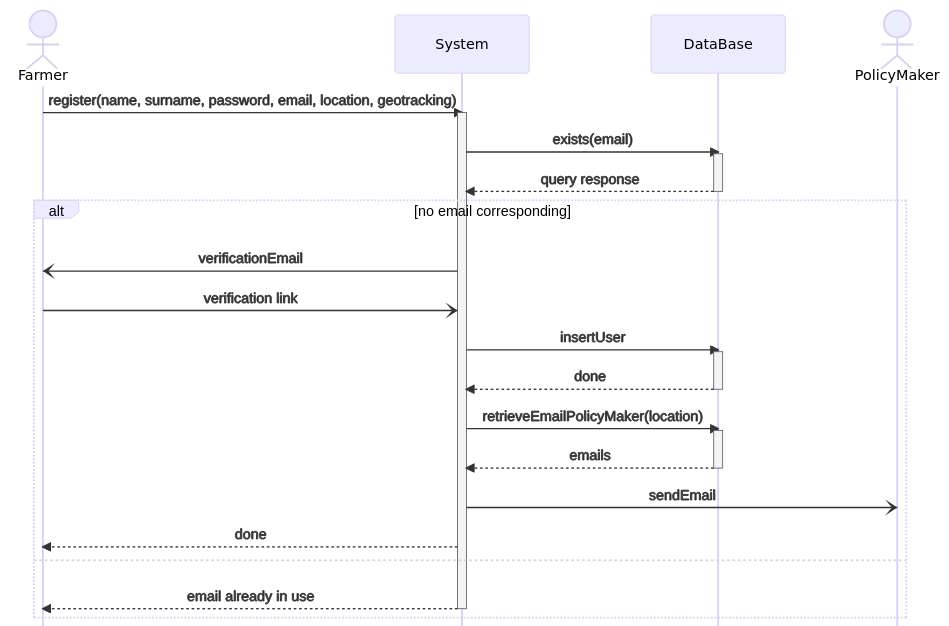
\includegraphics[width=\textwidth]{Images/seq_registration.png}
	\caption{\label{fig:seq_registration} Registration of a Farmer}
\end{figure}

\begin{figure} [!h]
	\centering
	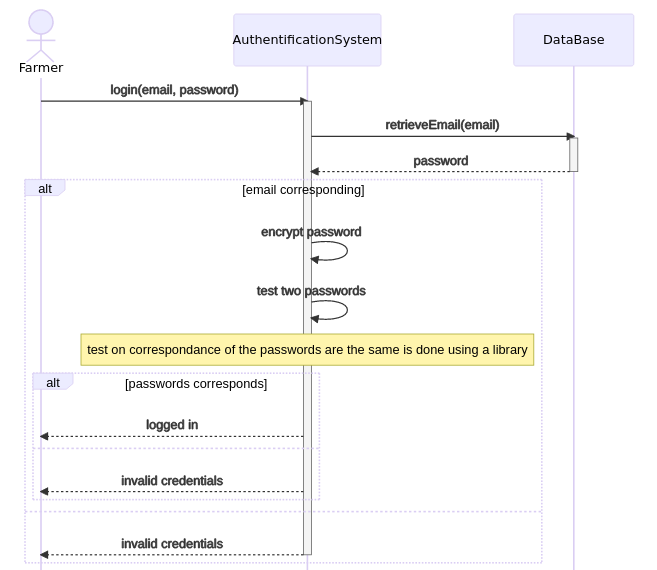
\includegraphics[width=\textwidth]{Images/seq_login.png}
	\caption{\label{fig:seq_login} Login of a Farmer}
\end{figure}

\begin{figure} [!h]
	\centering
	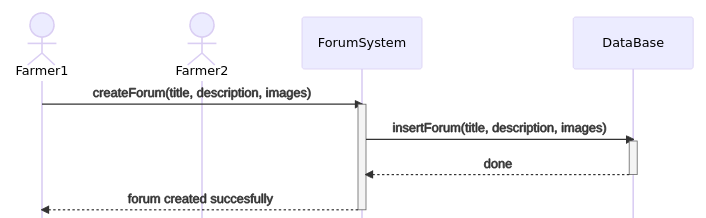
\includegraphics[width=\textwidth]{Images/seq_forum_creation.png}
	\caption{\label{fig:seq_crea_forum} Creation of a forum}
\end{figure}
